\begin{frame}<1-4|handout:1>[label=deeperPipeline]{deeper pipeline}
\countStyles
\circuitStyles
\begin{tikzpicture}
    \renewcommand{\plusTwo}{+4}
    \renewcommand{\plusOne}{+2}
    \timesThreePipeStuff
    \begin{pgfonlayer}{fg}
        \begin{scope}[every node/.style={color=red!70!black,ultra thick}]
        \node[hRegSmall={$A$ ($t+3$)},fill=white] at ([yshift=-.2cm]alu1.center |- alu2.-130) {};
            \node[hReg={$2\times A$ \\ partial results},fill=white] (split1) at (alu1.center) {};
            \alt<5-6|handout:2>{
                \node[opacity=0.2,hReg={},fill=white] (ghostSplit2) at (alu2.center) {};
                \node[color=red,hReg={$3\times A$ \\ partial results},fill=white] (split2) at ([xshift=.25cm]alu2.center) {};
            }{
                \node[hReg={$3\times A$ \\ partial results},fill=white] (split2) at (alu2.center) {};
            }
        \end{scope}
    \end{pgfonlayer}
    \coordinate (timelineBase) at ($(aInput.south)+(0cm,-2.5cm)$);
    \foreach \basis/\ref in {OneReg/aInput,OneHalfReg/split1,TwoReg/twoTimesReg,TwoHalfReg/split2,ThreeReg/threeTimesReg} {
        \coordinate (before\basis) at ([xshift=-.25cm]\ref.west);
        \coordinate (after\basis) at ([xshift=.25cm]\ref.east);
    }

    \foreach \basis/\alu/\reg in {OneAdd/alu1/OneHalfReg,TwoAdd/alu2/TwoHalfReg} {
        \coordinate (beforeHalf\basis) at ([xshift=-1cm]\alu.west);
        \coordinate (afterHalf\basis) at (before\reg);
        \coordinate (before\basis) at (after\reg);
        \coordinate (after\basis) at ([xshift=1cm]\alu.east);
    }
    \coordinate (timelineBaseLow) at ($(aInput.south)+(0cm,-3.5cm)$);
    \begin{visibleenv}<2-|handout:1>
    \foreach \basis/\len in {OneReg/$10$ ps,HalfOneAdd/$25$ ps,OneAdd/$25$ ps,OneHalfReg/$10$ ps,TwoReg/$10$ ps,HalfTwoAdd/$25$ ps,TwoHalfReg/$10$ ps,TwoAdd/$25$ ps,ThreeReg/$10$ ps} {
        \begin{scope}[very thick,Latex-Latex]
            \draw (before\basis |- timelineBase) -- (after\basis |- timelineBase)
                node[midway,below,font=\scriptsize] (timeline-\basis) {\len};
        \end{scope}
    }
    \end{visibleenv}
    \begin{visibleenv}<3|handout:1>
        \begin{scope}[overlay]
       \node[anchor=west] at ([yshift=-1cm]beforeOneReg |- timelineBaseLow) {exercise: throughput now?};
        \end{scope}
    \end{visibleenv}
    \begin{visibleenv}<4|handout:1>
        \iftoggle{heldback}{}{
        \begin{scope}[overlay]
        \draw[very thick,red,Latex-Latex] (beforeOneReg |- timelineBaseLow) -- (afterHalfOneAdd |- timelineBaseLow)
            node[below right, xshift=-2.5cm]{throughput: $\frac{1}{35 \text{ ps}} \approx 28$ G ops/sec};
        \end{scope}
        }
    \end{visibleenv}
    \begin{visibleenv}<5-6|handout:2>
        \begin{scope}[overlay]
        \node[cross out,red,thick,draw] (crossOut1) at (timeline-HalfTwoAdd.center) {};
        \node[below=0cm of crossOut1,red,font=\small] {30 ps};
        \node[cross out,red,thick,draw] (crossOut2) at (timeline-TwoAdd.center) {};
        \node[below=0cm of crossOut2,red,font=\small] {20 ps};
        \end{scope}
    \end{visibleenv}
    \begin{visibleenv}<5|handout:2>
        \begin{scope}[overlay]
            \node[anchor=west] at ([yshift=-1cm]beforeOneReg |- timelineBaseLow) {exercise: throughput now? (didn't split second add evenly)};
        \end{scope}
    \end{visibleenv}
    \begin{visibleenv}<6|handout:2>
        \iftoggle{heldback}{}{
        \begin{scope}[overlay]
        \draw[very thick,red,Latex-Latex] (beforeTwoReg |- timelineBaseLow) -- (afterHalfTwoAdd |- timelineBaseLow)
            node[below right, xshift=-2.5cm]{throughput: $\frac{1}{40 \text{ ps}} \approx 25$ G ops/sec};
        \end{scope}
        }
    \end{visibleenv}
\end{tikzpicture}
\begin{visibleenv}<7-|handout:3->
    \vspace{0cm}
    \begin{itemize}
        \item Problem: \myemph<7|handout:3>{How much faster can we get?}
        \item Problem: \myemph<8|handout:4>{Can we even do this?}
    \end{itemize}
\end{visibleenv}
\end{frame}

\againframe<7|handout:3>{deeperPipeline}

\begin{frame}[fragile,label=diminishDelay]{diminishing returns: register delays}
\begin{tikzpicture}
    \tikzset{
        logic/.style 2 args={draw,rectangle,align=center,anchor=north west,minimum width=#1,on chain,join,
                      inner sep=4pt,outer sep=1pt,minimum height=0.75cm,
                      label={[font=\small]-90:#2},fill=blue!30,font=\scriptsize},
        myl/.style 2 args={label={[align=right]180:#2 ps\\per cycle}},
        myReg/.style={hReg={10 ps},minimum height=0.75cm,on chain,join},
        every join/.style={-Latex,very thick},
        my chain/.style={start chain,node distance=5mm},
    }
    \matrix {
    \begin{scope}[my chain]
        \node[logic={5cm}{100 ps},myl={1 stage}{110}] {logic (all)};
        \node[myReg] {};
    \end{scope} \\
    \begin{scope}[my chain]
        \node[logic={2.5cm}{50 ps},myl={2 stage}{60}] {logic (1/2)};
        \node[myReg] {};
        \node[logic={2.5cm}{50 ps}] {logic (2/2)};
        \node[myReg] {};
    \end{scope} \\
    \begin{scope}[my chain]
        \node[logic={1.5cm}{33 ps},myl={5 stage}{43}] {logic (1/3)};
        \node[myReg] {};
        \node[logic={1.5cm}{33 ps}] {logic (2/3)};
        \node[myReg] {};
        \node[logic={1.5cm}{33 ps}] {logic (3/3)};
        \node[myReg] {};
    \end{scope} \\
    \begin{scope}[my chain, node distance=20mm, every node/.style={inner sep=0pt}]
        \node[on chain] {\vdots};
        \node[on chain] {\vdots};
        \node[on chain] {\vdots};
        \node[on chain] {\vdots};
    \end{scope}
    \\
    \begin{scope}[my chain,node distance=7mm]
        \node[logic={0.1cm}{1 ps},myl={100 stage}{11}] {\strut};
        \node[myReg] {};
        \node[logic={0.1cm}{1 ps}] {\strut};
        \node[myReg] {};
        \node[logic={0.1cm}{1 ps}] {\strut};
        \node[myReg] {};
        \node[logic={0.1cm}{1 ps}] {\strut};
        \node[myReg] {};
        \node[on chain,join] {\ldots};
    \end{scope} \\
    };
\end{tikzpicture}
\end{frame}

% FIXME: graph
\begin{frame}[fragile,label=regDelayLat]{diminishing returns: register delays}
\begin{tikzpicture}
\begin{axis}[width=.95\textwidth,height=0.8\textheight,xlabel={number of stages},ylabel={time per completion (ps)},
    xmin=0.5,xmax=15.5,ymin=0,ymax=120]
    \addplot[domain=1:15,samples=15,only marks,blue] {100/x+10}
        coordinate[pos=0] (t0)
        coordinate[pos=1/14] (t1)
        coordinate[pos=13/14] (t13)
        coordinate[pos=14/14] (t14);
    \path[name path=ten] (0,10) -- (16, 10);
    \path[name path=zero] (0,0) -- (16, 0);
    \only<2->{
        \addplot+[pattern=north west lines,opacity=0.2] fill between[of=ten and zero];
        \node[anchor=center] at (8,5) { register delay };
    }
    \only<3->{
        \draw[red] (t0) -| (t1) node[near start, right] {1.83x speedup};
        \draw[red] (t13) -| (t14) node[near start, above, xshift=-1cm] {1.02x speedup};
    }
\end{axis}
\end{tikzpicture}
\end{frame}

\begin{frame}[fragile,label=regDelayThru]{diminishing returns: register delays}
\begin{tikzpicture}
\begin{axis}[width=.95\textwidth,height=0.8\textheight,xlabel={number of stages},ylabel={throughput (ops/ns)},
    xmin=0.5,xmax=15.5,ymin=0,ymax=105]
    \addplot[domain=1:15,samples=15,only marks,blue] {1000/(100/x+10)}
        coordinate[pos=0] (t0)
        coordinate[pos=1/14] (t1)
        coordinate[pos=13/14] (t13)
        coordinate[pos=14/14] (t14);
    \draw[red] (t0) -| (t1) node[midway, right] {1.83x throughput};
    \draw[red] (t13) -| (t14) node[near start, above, xshift=-1.5cm] {1.02x throughput};
    \only<2->{
        \draw[red,dashed,line width=1pt] (0,100) -- (16,100)
            node[midway,below] {max. rate of register updates};
    }
\end{axis}
\end{tikzpicture}
\end{frame}

\againframe<8|handout:4>{deeperPipeline}

\againframe<5-6|handout:2>{deeperPipeline}

\begin{frame}[fragile,label=diminishSplit]{diminishing returns: uneven split}
\begin{itemize}
    \item Can we split up some logic (e.g. adder) arbitrarily?
    \item Probably not...
\end{itemize}
\begin{tikzpicture}
    \tikzset{
        logic/.style 2 args={draw,rectangle,align=center,anchor=north west,minimum width=#1,on chain,
                      inner sep=4pt,outer sep=1pt,minimum height=0.75cm,
                      label={[font=\small]-90:#2},fill=blue!30,font=\scriptsize},
        myl/.style 2 args={label={[align=right]180:#2 ps\\per cycle}},
        myReg/.style={hReg={10 ps},minimum height=0.75cm,on chain},
        every join/.style={-Latex,very thick},
        my chain/.style={start chain,node distance=0mm},
    }
    \matrix {
    \begin{scope}[my chain]
        \node[logic={5cm}{100 ps},myl={1 stage}{110}] {logic (all)};
        \node[myReg] {};
    \end{scope} \\
    \begin{scope}[my chain]
        \node[logic={3cm}{\myemph<2>{60 ps}},myl={2 stage}{70}] {logic (1/2)};
        \node[myReg] {};
        \node[logic={2.5cm}{\myemph<2>{45 ps}}] {logic (2/2)};
        \node[myReg] {};
    \end{scope} \\
    \begin{scope}[my chain]
        \node[logic={2cm}{\myemph<3>{40 ps}},myl={3 stage}{50}] {logic\\(1/3)};
        \node[myReg] {};
        \node[logic={2cm}{\myemph<3>{40 ps}}] {logic\\(2/3)};
        \node[myReg] {};
        \node[logic={1.5cm}{\myemph<3>{30 ps}}] {logic\\(3/3)};
        \node[myReg] {};
    \end{scope} \\
    \begin{scope}[my chain, node distance=20mm, every node/.style={inner sep=0pt}]
        \node[on chain] {\vdots};
        \node[on chain] {\vdots};
        \node[on chain] {\vdots};
        \node[on chain] {\vdots};
    \end{scope}
    \\
    };
\end{tikzpicture}
\end{frame}
